\documentclass[12pt]{article}

\usepackage{sbc-template}
\usepackage{graphicx,url}
\usepackage[utf8]{inputenc}
\usepackage[english]{babel}
\usepackage{float}
\usepackage{placeins}
%\usepackage[latin1]{inputenc}  

     
\sloppy

\title{A literature review on the embedded systems field applied to data collection-aided instrumentation for the Physics teaching lab}

\author{Victor Hugo Bitencourt\inst{1}}

\address{Universidade do Estado da Bahia -- Campus I
  (UNEB)\\
  41.150-000 -- Salvador -- BA -- Brazil
  \email{abjurandam@gmail.com}
}

\begin{document} 

\maketitle

\begin{abstract}
  A literature review was conducted to understand the embedded systems field applied to data collection-aided instrumentation for the Physics teaching lab. 
  Databases searched include IEEE Xplore and the European Journal of Physics, both last searched 2026, April 26.
  Exclusion criteria include little to no applicability in the physics teaching lab, and little to no instrumentation or embedded systems relevance.
  Risk of bias was assessed using methodological clarity and reproducibility, and results were synthesized with LLMs following manual human verification.
  51 papers were included.
  Findings indicate a gap between high-cost, high-precision instrumentation and low-cost, low-accuracy solutions, with few works addressing both affordability and measurement reliability thanks to the usage of custom experimentation setups with cheap embedded devices such as microcontrollers and sensors, and IoT-related connectivity.
  The evidence is limited by the time constraints to perform the review, which resulted in a low sample size of papers.
  The findings suggest that developing low-cost yet accurate instrumentations is needed in this domain, and wireless instrumentation is a possible high impact intervention in real physics teaching labs.
\end{abstract}

\section{Introduction}

This review was conducted with the aim to build knowledge about the proposed field.
Its unique value is summarizing the current state of the field in a trustable way through methodological rigor, bringing data to support a relevant intervention.
The starting point was the following intervention: ``a low-cost architecture using wireless connection to manage physics teaching experiments with a computer''.
Questions of the review include:

\begin{itemize}
  \item How do embedded systems aid data collection for educational physics experiments?
  \item How do web servers aid data telemetry from educational physics experiments?
  \item How does technology aid analysis of results from educational physics experiments?
  \item How does technology enhance learning in educational physics experiment laboratories?
\end{itemize}

\section{Methods}

The literature review process was aided by the Parsifal web research tool \cite{parsifal}, from paper importing, screening and data extraction recording. In all steps but data extraction of accepted papers, no AI tools were used, to minimize risk of bias and make the author accountable for it.

It was decided diverse databases that could provide papers with different angles to the research question would be the ideal choice for a reliable review. IEEE Xplore \cite{ieee} was the first database chosen, given its reputation for good engineering papers that could satisfy the aim of finding texts with satisfactory details in experimental architectures. The European Journal of Physics, accessed via the IOP Science platform \cite{iop}, was the second database chosen, for a physics and education-focused angle of the problem, thanks to its reputation in these fields. Last search date was April 26, 2026.

The search strategy was tuned given time constraints, aiming to narrow down the large scope of the field of physics education instrumentation by keywords more closely related to the proposed intervention carefully to avoid overly biased searched results. This was done by fitting the research questions in the PICOC framework \cite{wohlin2012experimentation}, which generate the search string via the Parsifal tool. The approach was tuning by the keywords until the generated search string returned a number of papers manageable for full text review, assuming most papers would pass the initial screening by title and abstract, as it is acceptable to happen in the rigorous review philosophy of seeking high recall \cite{cochrane_handbook_2024}. A search string that returned 174 papers in total accross both databases was deemed acceptable for providing a manageable volume of papers for a robust review.

The final search string was:

\begin{verbatim}
("educational laboratory" OR "physics education" 
OR "teaching laboratory") AND 
("Arduino" OR "data acquisition" OR "embedded system" 
OR "microcontroller") AND ("education" OR "learning" 
OR "low cost" OR "low-cost" OR "teaching")
\end{verbatim}

Other than search string tuning, selection was aided by the additional filter of papers after 2008. This decision was motivated by the fact that the Arduino Nano was released that year. Such microcontroller is currently the oldest widely sold board in the market created by the Arduino brand, which in turn is widely recognized as the most popular microcontroller brand.

Initial selection by title and abstract had the following exclusion criteria of each paper:

\begin{itemize}
  \item Does it not at least suggest experimental infrastructure?
  \item Does it not at least suggest a teaching lab?
  \item Is the experiment a virtual simulation instead of real experiment?
  \item Does it not at least suggest physics experiments?
\end{itemize}

The choice for permissive criteria in initial selection was taken to prioritize high recall.
Quality assessment by full text was not permissive, though. Said step had the following criteria for each paper:

\begin{itemize}
  \item Is it relevant to experimental instrumentation or embedded systems?
  \item Is there a clear contribution to experimental teaching methodology?
  \item Is there a physics teaching laboratory context?
  \item Is there an experimental activity involving students?
  \item Is there a data acquisition or measurement process?
\end{itemize}

Each full paper was assessed given this criteria with Yes/Partially/No values, after it was decided selected studies should have a score cutoff of 3.5. Careful reading of full text was needed to assess with minimal bias.

Lastly, accepted papers were uploaded in a LLM app for extraction of data fields, followed by human verification.

\section{Results}

From the two databases selected, 174 studies were found. 19 were excluded by paper and abstract, leaving 155 for quality assessment, which involved reading of full text. At this step, 97 studies were rejected and 26 were not found because due to no open access. In the end, 51 studies were included in the review.

\begin{figure}[H]
\centering
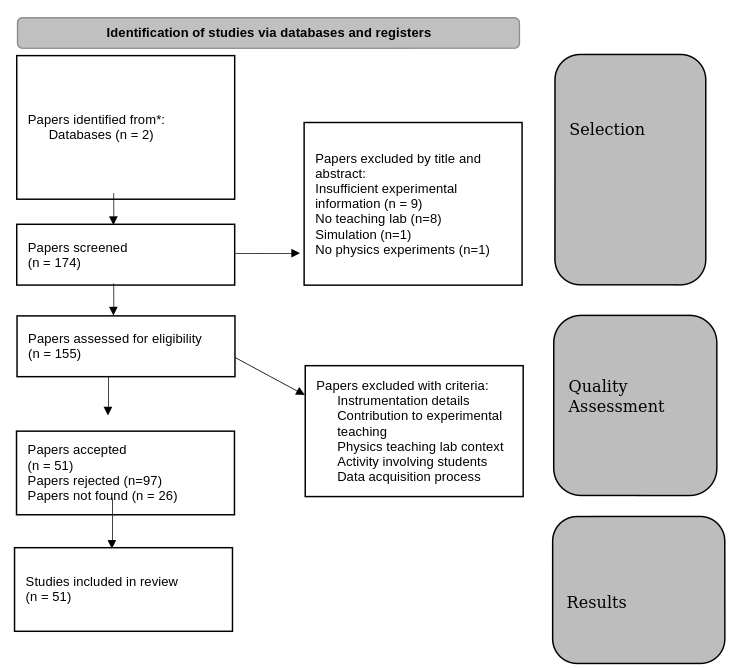
\includegraphics[width=.9\textwidth]{prismagray.png}
\caption{Paper screening strategy}
\label{fig:exampleFig1}
\end{figure}

Some studies might appear to meet the inclusion criteria, but were excluded because of lack of scoring in the chosen quality assessment approach.

During data extraction of accepted texts, studies were distinguished by three approaches: physics precision-first (precise instrumentation but high cost, or not friendly for individuals not from physics backgrounds), education learning-first (friendly for the genereal public but with low focus on precise instrumentation) and embedded/hybrid (with microcontrollers having the most representation). 

Quantitative patterns of studies were extracted via Python code.

\begin{figure}[H]
\centering
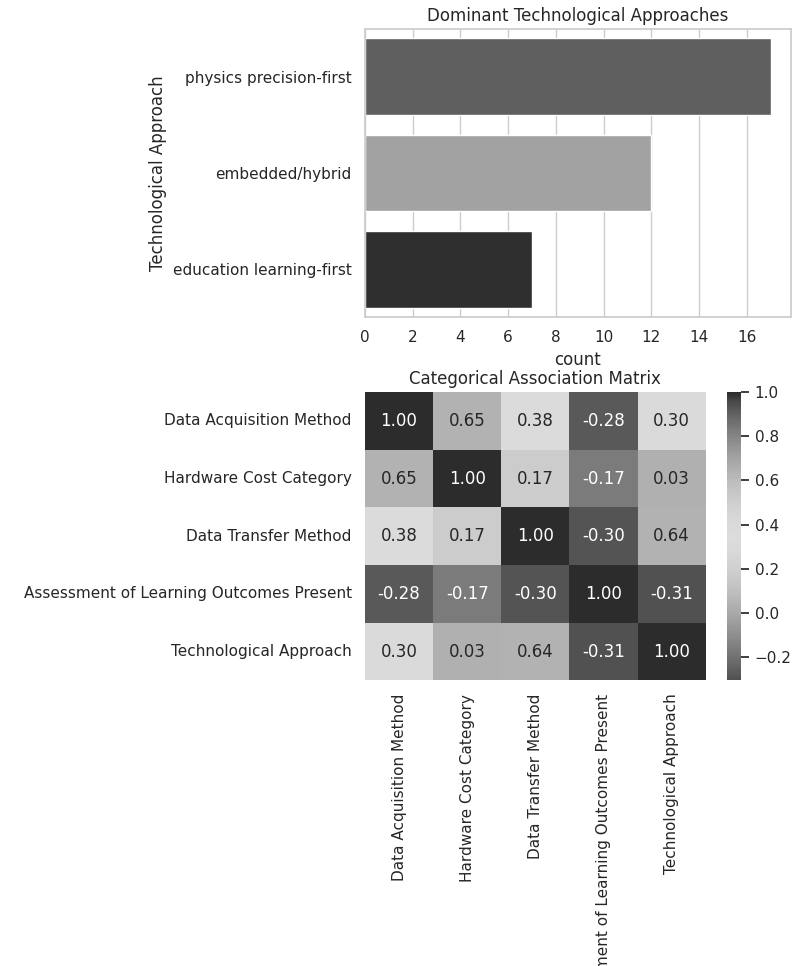
\includegraphics[width=.9\textwidth]{docmatrixgray.png}
\caption{Paper screening strategy}
\label{fig:exampleFig10}
\end{figure}

\section{Discussion}

Unlike initially thought, the embedded/hybrid approach wasn't as uncommon as expected, although still not as common as the physics precision-first approach. The results of Dominant Technological Approaches indicate a good representation of the need of best precision possible in such studies, given their respective constraints and methodological focus.

The Categorical Association Matrix of the data of accepted texts, created with a label encoder \cite{sklearn}, indicate a strong correlation of Data Acquisition Method and Hardware Cost Category, matching assumptions of the data acquisition method heavily influencing the total cost of experimental setup. There was a high correlation with data transfer method and technological approach too, matching initial assumptions of embedded setups dominating the representation of advanced approaches of data transfer, such as wireless connectivity.

The findings indicate a gap in the studies related with cheaper experimental setups with precise data logging, and confirm the proposed intervention of the usage of embedded systems as a high impact approach for making experimental data transfers cheap, scalable and easy to use.

\section{General Information}

All full papers and posters (short papers) submitted to some SBC conference,
including any supporting documents, should be written in English or in
Portuguese. The format paper should be A4 with single column, 3.5 cm for upper
margin, 2.5 cm for bottom margin and 3.0 cm for lateral margins, without
headers or footers. The main font must be Times, 12 point nominal size, with 6
points of space before each paragraph. Page numbers must be suppressed.

Full papers must respect the page limits defined by the conference.
Conferences that publish just abstracts ask for \textbf{one}-page texts.

\section{First Page} \label{sec:firstpage}

The first page must display the paper title, the name and address of the
authors, the abstract in English and ``resumo'' in Portuguese (``resumos'' are
required only for papers written in Portuguese). The title must be centered
over the whole page, in 16 point boldface font and with 12 points of space
before itself. Author names must be centered in 12 point font, bold, all of
them disposed in the same line, separated by commas and with 12 points of
space after the title. Addresses must be centered in 12 point font, also with
12 points of space after the authors' names. E-mail addresses should be
written using font Courier New, 10 point nominal size, with 6 points of space
before and 6 points of space after.

The abstract and ``resumo'' (if is the case) must be in 12 point Times font,
indented 0.8cm on both sides. The word \textbf{Abstract} and \textbf{Resumo},
should be written in boldface and must precede the text.

\section{CD-ROMs and Printed Proceedings}

In some conferences, the papers are published on CD-ROM while only the
abstract is published in the printed Proceedings. In this case, authors are
invited to prepare two final versions of the paper. One, complete, to be
published on the CD and the other, containing only the first page, with
abstract and ``resumo'' (for papers in Portuguese).

\section{Sections and Paragraphs}

Section titles must be in boldface, 13pt, flush left. There should be an extra
12 pt of space before each title. Section numbering is optional. The first
paragraph of each section should not be indented, while the first lines of
subsequent paragraphs should be indented by 1.27 cm.

\subsection{Subsections}

The subsection titles must be in boldface, 12pt, flush left.

\section{Figures and Captions}\label{sec:figs}


Figure and table captions should be centered if less than one line
(Figure~\ref{fig:exampleFig1}), otherwise justified and indented by 0.8cm on
both margins, as shown in Figure~\ref{fig:exampleFig2}. The caption font must
be Helvetica, 10 point, boldface, with 6 points of space before and after each
caption.

\begin{figure}[ht]
\centering
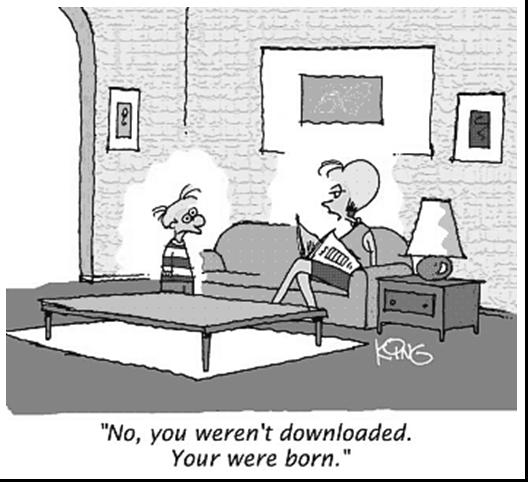
\includegraphics[width=.5\textwidth]{fig1.jpg}
\caption{A typical figure}
\label{fig:exampleFig1}
\end{figure}

\begin{figure}[ht]
\centering
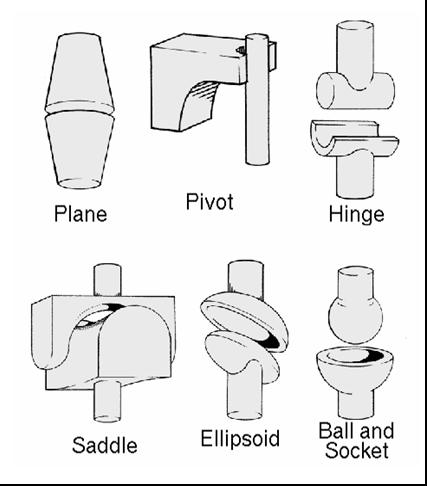
\includegraphics[width=.3\textwidth]{fig2.jpg}
\caption{This figure is an example of a figure caption taking more than one
  line and justified considering margins mentioned in Section~\ref{sec:figs}.}
\label{fig:exampleFig2}
\end{figure}

In tables, try to avoid the use of colored or shaded backgrounds, and avoid
thick, doubled, or unnecessary framing lines. When reporting empirical data,
do not use more decimal digits than warranted by their precision and
reproducibility. Table caption must be placed before the table (see Table 1)
and the font used must also be Helvetica, 10 point, boldface, with 6 points of
space before and after each caption.

\begin{table}[ht]
\centering
\caption{Variables to be considered on the evaluation of interaction
  techniques}
\label{tab:exTable1}
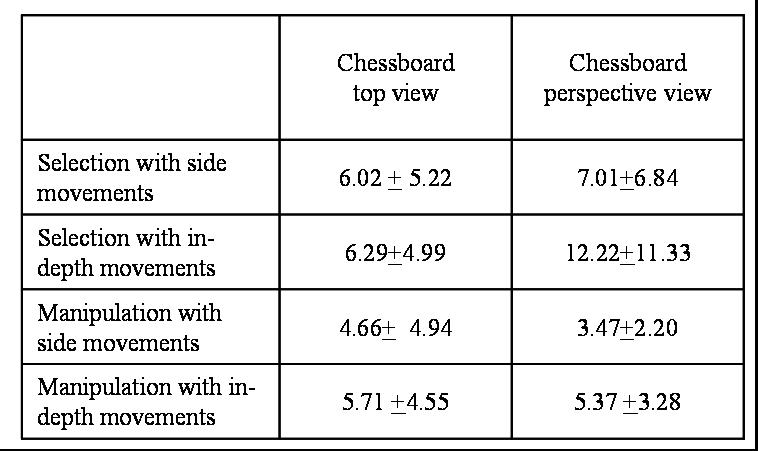
\includegraphics[width=.7\textwidth]{table.jpg}
\end{table}

\section{Images}

All images and illustrations should be in black-and-white, or gray tones,
excepting for the papers that will be electronically available (on CD-ROMs,
internet, etc.). The image resolution on paper should be about 600 dpi for
black-and-white images, and 150-300 dpi for grayscale images.  Do not include
images with excessive resolution, as they may take hours to print, without any
visible difference in the result. 

\bibliographystyle{sbc}
\bibliography{sbc-template}

\end{document}
